\documentclass[assd_tp2_main.tex]{subfiles}

\begin{document}

\section{Espectrograma}

\subsection{Funci\'on para realizaci\'on de espectrograma}

Para la realizaci\'on de los espectrogramas, se utiliz\'o la funci\'on ``spectrogram'', de la librer\'ia <<scipy>> de Python. La misma se basa en la implementaci\'on de transformadas de Fourier consecutivas sobre la se\~nal a lo largo del tiempo. La sintaxis para su utilizaci\'on es la siguiente:

\begin{center}
scipy.signal.spectrogram(x, fs=1.0, window=('tukey', 0.25), nperseg=None, noverlap=None, nfft=None, detrend='constant', return\_onesided=True, scaling='density', axis=-1, mode='psd')
\end{center}

Donde los par\'ametros y sus efectos en detalle se describen a continuaci\'on.

\begin{itemize}

\item \textbf{x [array]}: arreglo con los valores que toma la se\~nal en el tiempo (sobre los que se aplica la transformada de Fourier).

\item \textbf{fs [float]}: frecuencia de sampleo de la se\~nal $x(t)$. Por defecto normalizada: 1.0.

\item \textbf{window [string \'o tuple \'o array]}: ventana temporal a utilizar. Influye tanto el tipo de ventana como como el ancho de la misma.\par
Respecto al tipo de ventana, si se utiliza por ejemplo una ventana cuadrada, esta posee un corte abrupto. Si en dicha ventana no entra un n\'umero entero de per\'iodos de la se\~nal, se produce un corte abrupto.\par
Esto remite en la aparici\'on de otras componentes de alta frecuencia que antes no hab\'ia, lo que se conoce como <<fuga espectral>> (dado que la energ\'ia de los arm\'onicos principales se ``fuga'' a los otros arm\'onicos nuevos). Otras ventanas (como la Blackman-Harris) tienen un corte suave en los extremos (tienden a cero gradualmente), lo que minimiza la fuga espectral considerablemente.\par
El ancho de la ventana interviene en la resoluci\'on en tiempo y en frecuencia. Si la ventana es m\'as ancha, se obtiene mayor resoluci\'on en frecuencia, dado que si la frecuencia de la se\~nal sufre alg\'un cambio en el tiempo (como en una se\~nal FM), es posible captarlo con la ventana con mayor definici\'on. Pero en el tiempo se pierde resoluci\'on dado que se sabe con menor precisi\'on d\'onde ocurre exactamente el cambio de frecuencia. Con una ventana angosta, se gana resoluci\'on en el tiempo, pero en frecuencia se podr\'ia perder el cambio que antes se lograba captar en el tiempo con una ventana ancha, por lo que se ver\'ia una sola frecuencia en lugar de dos.

\item \textbf{npersec [int]}: es el largo de cada segmento. Por defecto es <<None>>, pero si la ventana se da en formato de <<string>> se considera 256, y si se da como <<array>> es el largo del mismo.

\item \textbf{noverlap [int]}: es el n\'umero de puntos a solapar entre segmentos. Por defecto es <<None>>, que es npersec // 8. Es decir, define la separaci\'on resultante entre ventanas.

\item \textbf{nfft [int]}: es el largo de la FFT utilizada. Por defecto es <<None>>, que determina el largo igual a ``npersec''.

\item \textbf{detrend [string \'o function \'o False]}: elimina la tendencia lineal a lo largo del eje temporal. Por defecto es ``constant''. Si es de tipo string, se pasa directamente a la funci\'on <<detrend>> (tambi\'en de scipy), y si es una funci\'on, se le pasa un segmento y lo devuelve ya con el dsv\'io correspondiente. Si es <<False>>, no se aplica ning\'un desv\'io. Para el caso de audio, no nos es de inter\'es.

\item \textbf{return\_ onesided [bool]}: si se asigna <<True>>, se devuelve un espectro unilateral. Si es <<False>>, el espectro ser\'a bilateral.

\item \textbf{scaling [‘density’, ‘spectrum’]}: considerando a $x(t)$ en volts [V], se elije si procesar la densidad espectral de potencia [$\textrm{V}^2/Hz$] \'o el espectro de potencia [$\textrm{V}^2$]. Por defecto se procesa la densidad espectral. Se simboliza como $S_{xx}$.

\item \textbf{axes [int]}: es el eje a lo largo del cual se procesa el espectrograma. Por defecto es <<-1>> (es decir, el \'ultimo utilizado).

\item \textbf{mode [str]}: define que es lo que se espera que devuelva la funci\'on, entre [``psd'', ``complex'', ``magnitude'', ``angle'', ``phase'']. ``psd'' es la densidad espectral de potencia; con ``complex'' devuelve la STFT (Short-Time Fourier Transform) compleja; ``magnitude'' devuelve el valor absoluto de la STFT, y ``angle'' y ``phase'' el \'angulo correspondiente complejo.

\end{itemize}

Los par\'ametros que devuelve son los siguientes:

\begin{itemize}

\item \textbf{f [ndarray]}: arreglo de dimensi\'on ``n'' con las frecuencias de sampleo.

\item \textbf{t [ndaray]}: arreglo de dimensi\'on ``n'' con los segmentos de tiempo.

\item \textbf{$S_xx$ [ndarray]}: arreglo de dimensi\'on ``n'' con el espectrograma de $x(t)$.

\end{itemize}

En referencia a las diferentes ventanas utilizables, adem\'as del ancho se debe considerar realizar el an\'alisis con o sin overlap (solapamiento entre segmentos). En el caso m\'as sencillo, no utilizar overlap podr\'ia conllevar p\'erdidad de informaci\'on: si se tiene un cambio de frecuencia de corta duraci\'on en comparaci\'on a la duraci\'on total del segmento, y se encuentra cerca del final de \'este, al no utilizar segmentos solapados para la STFT podr\'ia perderse dicho evento. Para evitar dicha p\'erdida de informaci\'on, se aplica la STFT a segmentos con un cierto grado de solapamiento. Se gana en no perder informaci\'on, pero se requiere mayor tiempo de procesamiento, dado que al ser segmentos solapados, para cubrir la totalidad de la se\~nal se necesita realizar m\'as veces la transformaci\'on. El porcentaje de overlap se encuentra en general entre el 50\% y el 75\%, de acuerdo al paper <<\textit{On the Use of Windows for Harmonic Analysis with the Discrete Fourier Transform}>> (1978, Fredric J. Harris, member IEEE).

\subsection{Aplicaci\'on a escala de Sol Mayor (G3)}

La tonalidad de \textit{sol} mayor (en el sistema ingl\'es abreviada como \textbf{G}) consiste en la escala mayor del sol y contiene las notas \textit{sol, la, si, do, re, mi, fa} sostenido y \textit{sol}. La notaci\'on \textbf{G3} corresponde a la peque\~na octava, cuya frecuencia es aproximadamente 195.998Hz.\par
El espetrograma realizado se muestra a continuaci\'on.

\begin{figure}[ht]	
\begin{centering}
	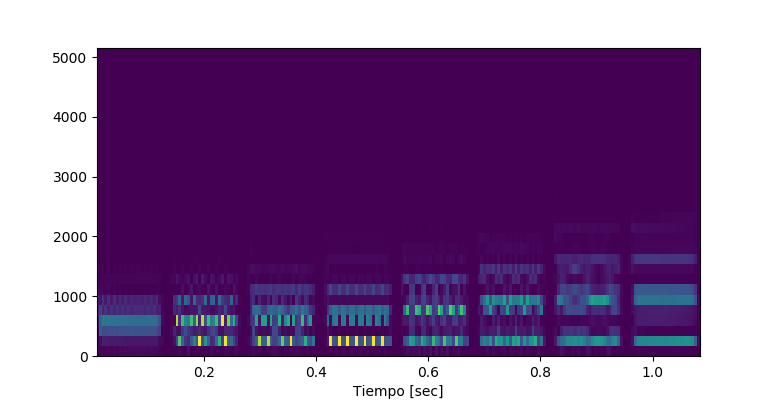
\includegraphics[scale=0.7]{graficos/Espectrograma7.png}
	\caption{Espectrograma de Sol mayor}
	\end{centering}\par
\end{figure}

En el espectrograma obtenido sintetizando con un piano, resulta visible la frecuencia de la primera octava cercana a los 200Hz. Se utilzan 120ms por nota seg\'un lo sugerido, de manera tal que puede diferenciarse cada una por la escala creciente en frecuencia.

\end{document}

